\providecommand{\main}{..}
\documentclass[\main/main.tex]{subfiles}

\colorlet{punct}{red!60!black}
\definecolor{background}{HTML}{EEEEEE}
\definecolor{delim}{RGB}{20,105,176}
\colorlet{numb}{magenta!60!black}

\lstdefinelanguage{json}{
    basicstyle=\normalfont\ttfamily,
    numbers=left,
    numberstyle=\scriptsize,
    stepnumber=1,
    numbersep=8pt,
    showstringspaces=false,
    breaklines=true,
    frame=lines,
    backgroundcolor=\color{background},
    literate=
     *{0}{{{\color{numb}0}}}{1}
      {1}{{{\color{numb}1}}}{1}
      {2}{{{\color{numb}2}}}{1}
      {3}{{{\color{numb}3}}}{1}
      {4}{{{\color{numb}4}}}{1}
      {5}{{{\color{numb}5}}}{1}
      {6}{{{\color{numb}6}}}{1}
      {7}{{{\color{numb}7}}}{1}
      {8}{{{\color{numb}8}}}{1}
      {9}{{{\color{numb}9}}}{1}
      {:}{{{\color{punct}{:}}}}{1}
      {,}{{{\color{punct}{,}}}}{1}
      {\{}{{{\color{delim}{\{}}}}{1}
      {\}}{{{\color{delim}{\}}}}}{1}
      {[}{{{\color{delim}{[}}}}{1}
      {]}{{{\color{delim}{]}}}}{1},
}

\begin{document}
\chapter{Methods}
\label{methods}
In this chapter is explained the finality of each service. Due to legal reasons in this manuscript there won't be any code or dataset example. Each service component will be explained through a pseudocode representation in order to make the whole system more understandable.\\
All services are Jupyter notebooks that exploit the parallelization ability of PySpark, working on several rows at the same time using MapReduce approach which is the \emph{de facto} standard in big data field.
\section{Preprocessing}
As said in Chapter 3, this is the phase where the dataset is elaborated in order to be used further on. 
\subsection{Cleaning}
Given a textual dataset, cleaning service performs all the operations needed to have cleaned and well formed documents.
\subsubsection{HTML cleaning}
The first (parametrized) step is to remove all HTML special characters. This operation is preparatory for next phases that need to deal with human-readable texts. The pseudocode of HTML removal phase is visible in Algorithm \ref{alg_html_removal}. This service is based on Python HTML class \cite{html_parser}, which allows to parse textual files filled with HTML special characters and tags.
\begin{center}
    \begin{algorithm}[H]
     \KwData{Textual dataset}
     \KwResult{Cleaned texts}
     initialization \\
     \ForEach{dataset row}{
      read document body \\
      unescape HTML special tags \\
      substitute resulting HTML tags with an empty string
     }
     \caption{HTML removal}
     \label{alg_html_removal}
    \end{algorithm}
\end{center}

\subsubsection{Sentence splitting}
This is the first step to overcome transformer technology limitations: in order to not increase to much memory usage, transformers libraries set a maximum of tokens that the model is able to manage. Therefore, long texts are difficult to manage as a whole, so they need to be divided in sentences (splits). In \mbox{Algorithm \ref{alg_split}} is visible the pseudocode for splitting phase.
\begin{center}
    \begin{algorithm}[H]
     \KwData{Cleaned dataset}
     \KwResult{Splitted texts}
     initialization \\
     \ForEach{dataset row}{
      read document body \\
      split text according to a regular expression
     }
     \caption{Text split}
     \label{alg_split}
    \end{algorithm}
\end{center}
\subsubsection{Split cleaning}
In order to obtain the best vectorial representation using transformers, splits need to be cleaned from all punctuation and special characters that are not truly useful. Those characters could be present in text due to human errors, OCR errors or even errors in format-to-format conversion. In Algorithm \ref{alg_split_cleaning} is visible the pseudocode for split cleaning operation.
\begin{center}
    \begin{algorithm}[H]
     \KwData{Splitted dataset}
     \KwResult{Cleaned splits}
     initialization \\
     \ForEach{dataset row}{
      read document splits \\
      \ForEach{split}{
        remove all useless punctuation \\
        remove all useless characters \\
        split in words \\
        \If{word is all uppercase}{
            convert to lowercase \\
            }
        \Else{keep the word}
        rebuild the sentence
      }
     }
     \caption{Split cleaning}
     \label{alg_split_cleaning}
    \end{algorithm}
\end{center}
\subsubsection{Split filtering}
The final step of cleaning service is split filtering. In this phase, splits that do not satisfy certain conditions (splits too short, splits too long, splits with too many repeated words, \dots) are filtered out in order to keep only correct splits. In Algorithm \ref{alg_split_filtering} is visible the pseudocode for split filtering operation. 
\begin{center}
    \begin{algorithm}[H]
     \KwData{Cleaned dataset}
     \KwResult{Filtered texts}
     initialization \\
     \ForEach{dataset row}{
      read document splits
      \ForEach{split}{
        \If{split is longer than threshold AND split length/number of word ratio is bigger than threshold}{
            keep split
            }
        \Else{filter out split}
      }
     }
     \caption{Split filter}
     \label{alg_split_filtering}
    \end{algorithm}
\end{center}

\subsection{Filtering}
In some applications, it is needed to reduce the number of records inside a dataset. In the implemented framework this is performed using the filtering service. Reading a list of keys which has to be kept, this service is able to filter out those keys that aren't part of the list mentioned earlier. Algorithm \ref{alg_filtering} shows how two datasets are joined in order to filter the bigger one. This operation is simply an inner join between two datasets resulting in a smaller dataset due to the filter one.
\begin{center}
    \begin{algorithm}[H]
     \KwData{Cleaned dataset}
     \KwData{Filter dataset}
     \KwResult{Filtered dataset}
     initialization \\
     join cleaned and filter dataset \\
     \Return filtered dataset with rows that are part of both datasets
     \caption{Dataset filter}
     \label{alg_filtering}
    \end{algorithm}
\end{center}

\section{Processing}
This category includes services that generate the information needed to perform all similarity tasks of the framework. Ideally, these services work on a cleaned dataset, so they are the next step of preprocessing services. 
\subsection{Embedding extraction}
This service is the core of the framework: decisions made in this service constitute the biggest discriminant of the framework. Using a given model, it converts sentences into vectorial representations (embedding). This is possible using a library called SentenceTransformers \cite{sbert}, based on their original work \emph{Sentence-BERT: Sentence Embeddings using Siamese BERT-Networks} \cite{reimers2019sentencebert}. SentenceTransformers allows to choose a transformer model from either the library itself or from another repository of transformer models: \emph{Huggingface} \cite{huggingface}. Here below is visible the list of Transformer families with a short description that have been used during the project:
\begin{enumerate}
    \item \textbf{BERT};
    \item \textbf{ALBERT};
    \item \textbf{DistilBERT};
    \item \textbf{MPNET};
    \item \textbf{XLM}.
\end{enumerate} 
\paragraph{BERT}
BERT has been the first transformer model released after Vaswani's \cite{vaswani2017attention}. It has been released and open sourced by Google, reaching the state-of-the-art for NLP. Reading this Google post \cite{bert_blog_post}, BERT can represent a word using its surrounding scope, contextualizing the representation. BERT has been the first deeply bidirectional, unsupervised language representation, pretrained using only a plain text corpus \cite{DBLP:journals/corr/abs-1810-04805}.
\paragraph{ALBERT}
Like BERT, ALBERT has been released by Google. Looking at this blog post by Google \cite{albert_blog_post}, ALBERT implements two main design changes respecting to BERT, in order to optimize the performances. The first change is to factorize the embedding parametrization, splitting the embedding matrix between input-level embeddings with a relatively-low dimension, while the hidden-layer embeddings use higher dimensionalities. The second aspect on which ALBERT focuses is layer stacking: differently from BERT, in ALBERT there is a parameter sharing across the layers, resulting in a slightly diminished accuracy while reducing the size of the model \cite{DBLP:journals/corr/abs-1909-11942}.
\paragraph{MPNET}
MPNET has been released by Microsoft in 2020. As visible from their blog post \cite{mpnet_blog_post},  researchers that developed MPNET, realized that two of the main pretraining tasks of transformers, masked language modeling adopted in BERT and permuted language modeling adopted in XLNet \ref{Yang2019XLNetGA} --- another transformer model presented by Google and Carnegie Mellon University researchers from which MPNET inherits ---, have different limitations. They came up with and approach that inherits the advantages of Masked language modeling (MLM) and Permuted language modeling (PLM) and avoids their limitations. MLM is proposed in BERT, which randomly masks some tokens with a masked symbol [M] and predicts the masked tokens given remaining tokens. PLM is proposed in XLNet, which randomly permutes a sequence and predicts the tokens in the right part (predicted part) in an autoregressive way. PLM can model the dependency among the predicted tokens with autoregressive prediction, but it cannot see the position information of the full sentence, which will cause mismatches between the pretraining and fine-tuning since the position information of the full sentence can be seen in the downstream tasks. MPNet uses masked and permuted language modeling to model the dependency among predicted tokens and see the position information of the full sentence \cite{DBLP:journals/corr/abs-2004-09297}.
\paragraph{DistilBERT}
DistilBERT has been released by HuggingFace engineers in 2019. They focused on the problem of growing model size and how to put in production such models. From the post on Huggingface blog \cite{distilbert_blog_post}, they used the \emph{distillation} technique to compress a large model into a smaller model.\\
\textbf{Distillation}: Knowledge distillation (sometimes also referred to as teacher-student learning) is a compression technique in which a small model is trained to reproduce the behavior of a larger model (or an ensemble of models). It was introduced by Bucila et al. \cite{10.1145/1150402.1150464} and generalized by Hinton et al. \cite{hinton2015distilling} a few years later \cite{DBLP:journals/corr/abs-1910-01108}.
\paragraph{XLM}
XLM transformer has been released by Facebook, in 2019 \cite{DBLP:journals/corr/abs-1901-07291}. As visible Facebook blog post \cite{xlm_blog_post}, researchers at Facebook developed this transformer model to extend the pretraining for English language to other languages. XLM uses a known pre-processing technique and a dual-language training mechanism with BERT in order to learn relations between words in different languages. First, instead of using word or characters as the input of the model, it uses Byte-Pair Encoding (BPE) that splits the input into the most common sub-words across all languages, thereby increasing the shared vocabulary between languages. Furthermore, it extends BERT architecture in the following two ways.
\begin{enumerate}
    \item Each training sample consists of the same text in two languages, whereas in BERT each sample is built from a single language. As in BERT, the goal of the model is to predict the masked tokens, however, with the new architecture, the model can use the context from one language to predict tokens in the other, as different words are masked words in each language (they are chosen randomly).
    \item The model also receives the language ID and the order of the tokens in each language, i.e. the Positional Encoding, separately. The new metadata helps the model learn the relationship between related tokens in different languages.
\end{enumerate}


SentenceTransformers abstracts all the tokenization and averaging logics: given a sentence, it is tokenized, for each token it is extracted a n-dimensional vector (e.g. $[1, 768]$) and finally those vectors are averaged in order to obtain a single n-dimensional vector. To overcome the problem of transformer model longest manageable sequence, the service performs a tokenization, using the model tokenizer, in order to check if the input sentence is manageable by the chosen model. If it's longer, the sentence is splitted in order to perform the extraction without any problem. The pseudocode is visible in Algorithm \ref{alg_embedding_extraction}:
\begin{center}
    \begin{algorithm}[H]
     \KwData{Cleaned dataset}
     \KwResult{Filtered dataset}
     initialization \\
     \ForEach{document split}{
        \If{split length > threshold}{
            further split \\
            splits embedding extraction
            }
        \Else{
            split embedding extraction
            } 
        }
     \Return embedded dataset
     \caption{Embedding extraction}
     \label{alg_embedding_extraction}
    \end{algorithm}
\end{center}

\subsection{Numerosity reduction}
Working with long documents ends up in having very long sets of vectors: their dimension remains the same because every extraction is performed with the same model, but their numerosity may vary: a document with 10 sentences has 10 different vectors, and so on. Depending on the model used, these vectors may increase the memory size of the document in a consistent way. To tackle this problem, we proposed and implemented a technique of vector numerosity reduction: in this way it's possible to reduce the memory consumption sacrificing some informative content. The implemented algorithm inside the framework is a service that exploits cosine similarity in order to reduce the vector number: after computing the internal similarity of the cartesian product of all sentences inside a document, the minimum spanning tree is extracted as follows. Every sentence is considered a node in a fully connected graph, while the edges are weighted with the cosine similarity value between the two sentences. The minimum spanning tree defines the path to follow in order to find highly similar sentences: if two sentences are similar over a given threshold, the two vectors are merged reducing the numerosity. \\
\textbf{Graph}: a graph is a diagram of vertices or nodes connected by edges \cite{Siu1998IntroductionTG}. \\
\textbf{Fully connected graph}: a fully connected graph is a graph in which every node is connected to every other node \cite{Siu1998IntroductionTG}. \\
\textbf{Tree}: a tree is a structure consisting of one node called the root and zero or more subtrees \cite{tree_definition}.

\textbf{Matrix representation}: 
Given a graph G with vertices labelled {1, 2, ..., $n$}, its \emph{adjacency matrix} A, visible in Figure \ref{adjacency_matrix_graph}, is a $n \times n$ matrix whose $ij$-th entry is the number of edges joining vertex i and vertex j. If, in addition, the edges are labelled {01, 12, 23,... , $nm$}, its \emph{incidence matrix} M, visible in Figure \ref{incidence_matrix_graph}, is the $n \times m$ matrix whose $ij$-th entry is 1 if vertex $i$ is incident to edge $j$, and 0 otherwise. If the edges have a weight, its \emph{weight matrix} W, visible in Figure \ref{weight_matrix_graph}, is the $n \times n$ matrix whose $ij$-th entry is the weight of the edge connecting vertex $i$ and vertex $j$.
\begin{figure}[H]
\centering
    \begin{tabular}{c c}{
        $\displaystyle
            A = 
        \renewcommand{\kbldelim}{(}% Left delimiter
        \renewcommand{\kbrdelim}{)}% Right delimiter
        \kbordermatrix{
            & 0 & 1 & 2 & 3 & \\
            0 & 0 & 1 & 0 & 1 \\
            1 & 1 & 0 & 1 & 0 \\
            2 & 0 & 1 & 0 & 1 \\
            3 & 1 & 0 & 1 & 0 \\
          }
        $}
        &
        $\vcenter{\hbox{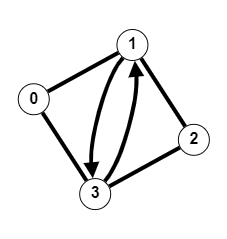
\includegraphics[scale=0.55]{images/methods/fully_connected_graph_adjacency.png}}}$
    \end{tabular}
    \caption{Graph corresponding to adjacency matrix A}
    \label{adjacency_matrix_graph}
\end{figure}

\begin{figure}[H]
\centering
    \begin{tabular}{c c}
        {$\displaystyle
            M = 
        \renewcommand{\kbldelim}{(}% Left delimiter
        \renewcommand{\kbrdelim}{)}% Right delimiter
          \kbordermatrix{
            & 01 & 12 & 23 & 30 & 02 & 13\\
            0 & 1 & 0 & 0 & 1 & 1 & 0\\
            1 & 1 & 1 & 0 & 0 & 0 & 1\\
            2 & 0 & 1 & 1 & 0 & 1 & 0\\
            3 & 0 & 0 & 1 & 1 & 0 & 1\\
          }$}
        &
        $\vcenter{\hbox{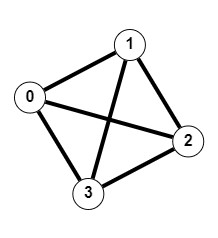
\includegraphics[scale=0.65]{images/methods/fully_connected_graph_example.png}}}$
    \end{tabular}
    \caption{Graph corresponding to incidence matrix M}
    \label{incidence_matrix_graph}
\end{figure}

\begin{figure}[H]
\centering
    \begin{tabular}{c c}
        {
        $\displaystyle
            W = 
        \renewcommand{\kbldelim}{(}% Left delimiter
        \renewcommand{\kbrdelim}{)}% Right delimiter
        \kbordermatrix{
            & 0 & 1 & 2 & 3 & \\
            0 & 0 & 0.2 & 0.60 & 0.40 \\
            1 & 0.20 & 0 & 0.25 & 0.35 \\
            2 & 0.60 & 0.25 & 0 & 0.15 \\
            3 & 0.40 & 0.35 & 0.15 & 0 \\
          }
        $}
        &
        $\vcenter{\hbox{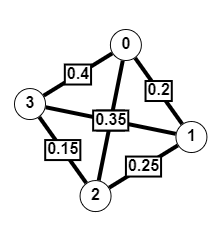
\includegraphics[scale=0.65]{images/methods/fully_connected_graph_weighted.png}}}$
    \end{tabular}
    \caption{Graph corresponding to weight matrix W}
    \label{weight_matrix_graph}
\end{figure}

\textbf{Minimum spanning tree}: An edge-weighted graph is a graph where we associate weights or costs with each edge. The spanning tree of a graph (G) is a subset of G that covers all of its vertices using the minimum number of edges. A graph can have more than one spanning tree. A minimum spanning tree (MST) \cite{books/daglib/0029345} of an edge-weighted graph is a spanning tree whose weight (the sum of the weights of its edges) is no larger than the weight of any other spanning tree. The pseudocode for numerosity reduction algorithm is visible in Algorithm \ref{alg_numerosity_reduction}.
\begin{center}
    \begin{figure}[h]
    \centering
    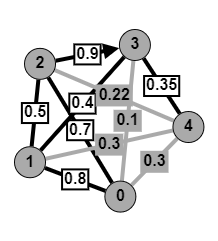
\includegraphics[scale=1.25]{images/methods/mst_example.png}
    \caption{MST example}
    \label{fig:mst_example}
\end{figure}
\end{center}
\begin{center}
    \begin{algorithm}[H]
     \KwData{Embedded dataset}
     \KwResult{Reduced dataset}
     initialization \\
     weight matrix calculation \\
     MST computation \\
     \ForEach{edge in MST}{
        \If{edge weight > similarity threshold}{
            merge similar sentence embeddings \\
            recompute weight matrix \\
            recompute MST
            }   
        }
     \Return filtered dataset with rows that are part of both datasets
     \caption{Numerosity reduction}
     \label{alg_numerosity_reduction}
    \end{algorithm}
\end{center}
In order to be able to perform this reduction, in this framework it is used \emph{SciPy} \cite{2020SciPyNMeth} package with its features: to compute the weight matrix is used \emph{cosine\_distances} method, while for MST computation is used \emph{minimum\_spanning\_tree} method.
\subsection{Similarity scoring}
In order to complete a similarity search task, a way of scoring this similarity is needed. The generated embeddings as terms of a given similarity function. 
\subsubsection{Long documents problem}
Working with long documents is not trivial, due to intrinsic limitations of transformer models. As said, each model has an input sequence maximum length that cannot be exceeded because it will lead to errors in vectorized representation (sequence truncation, exception raising, \dots). A possible solution to this problem could be averaging all the vectors of different sentences that constitute the original text. The higher the number of sentences, the higher the information dilution: the final vector will be a vector that doesn't truly represent anything inside the original text, leading to high similarity scores even if the original documents are very different. In the next subsection will be presented the chosen similarity scoring approach.
\subsubsection{Similarity scoring algorithm}
As previously mentioned, working with long documents is not that easy. Starting from the cleaning phase where text bodies are divided in sentences, it has been decided to use a \emph{voting} approach. The voting approach allows to compare documents using the sentences that compose them, allowing in this way to let each sentence "choose" its most similar sentence from other document. The similarity is calculated using cosine similarity, which has been observed to work well in semantic similarity fields. The choice of the most similar sentence is performed keeping the highest scoring sentence in the research document and its score. To give a final result, the algorithm summarizes a resulting score computing one last operation (mean, median, ...) on the list of highest scoring sentences scores chosen by query sentences. The service produces a \emph{result dataset} with rows built like Listing \ref{ex_param_msg}:
\\
\begin{center}
    \begin{lstlisting}[language=json, caption="Parameter message example", captionpos=b, label={ex_param_msg}]
        {
         "query_document_key": "query_key",
         "search_document_key": "search_key",
         "score": 0.8
        }
    \end{lstlisting}
\end{center}
The pseudocode is visible in Algorithm \ref{alg_scoring}.
\begin{center}
    \begin{algorithm}[H]
     \KwData{Query document}
     \KwData{Search document}
     \KwResult{Scores dataset}
     initialization\\
     \ForEach{sentence in query document}{
        \ForEach{sentence in search document}{
            compute cosine similarity 
            }
        choose most similar sentence
        }
     compute final score\\
     \Return score
     \caption{Scoring algorithm}
     \label{alg_scoring}
    \end{algorithm}
\end{center}

\section{Evaluation}
After computing all necessary scores, in order to understand if the hyperparameters configuration works well it's essential to define an evaluation method. The evaluation method is mandatory in order to have a reliable set of hyperparameters. \\
\subsection{Baseline dataset}
In order to perform an evaluation, a baseline dataset must be defined. The baseline dataset used throughout the project is constituted by 10 query documents and each one has associated 10 search documents: of these 10 documents, 5 are adherent to the query and 5 are not adherent.
\subsection{Evaluation method}
To understand if the framework is working well, it has been decided to focus on two main aspects:
\begin{enumerate}
    \item \textbf{Classification precision}: the first aspect to consider is if the framework is able to give back the same results that a human would give back to a query search;
    \item \textbf{Difference between right and wrong}: the second aspect to consider is how differently the system scores right and wrong search documents.
\end{enumerate}
\subsubsection{Evaluation metrics}
\paragraph{Precision@n} In order to understand how precise is the framework, it has been used an evaluation metric called \emph{precision}: recalling the structure of the baseline dataset, where there are 5 correct documents and 5 incorrect documents for each query, the computed scores are ordered in descending order: the number of correct placed documents (first half for adherent documents, second half for non adherent documents) denotes the precision for that given query. Precision denotes the proportion of predicted positive cases that are correctly Real Positives \cite{DBLP:journals/corr/abs-2010-16061}.\\
As the name says, Precision@n is an evaluation metric computed on the $n$ corpus elements: for a given query the resulting measure is \emph{precision@10}, where 10 are the documents associated to the given query. For a given set of queries with two groups of mutually exclusive documents associated (\emph{related}, \emph{not related}), the final result will be the sum of these precisions: for example, for 10 queries there will be a \emph{precision@100} score.
\paragraph{Difference mean/median} The other aspect which deserves particular attention is the difference between right and wrong documents. In order to have a reliable framework, it's necessary not only that it assigns right documents to right queries, it would be better if it could be able to strongly differentiate right documents from wrong ones. In order to measure this metric, the system performs the mean of median of similarity scores assigned to right documents in baseline and computes the difference with the mean or median form wrong ones: the higher the difference, the better the result. An high score for these metrics would mean that the system can well recognize right documents, resulting in a more reliable result. 
\end{document}